\chapter{Radiative Transfer and Ionization}

\epigraph{``I'm splashing greys where once was glowing white''}{{\sl Mike Vennart, Silent/Transparent}}

In the previous chapters I have given an introduction to the field and 
some relevant background relating to accretion 
discs and their associated outflows. Now it proves useful
to discuss some of the specific {\em methods} one might be able to use
in order to answer some of the questions raised in the previous sections.
In particular, I will discuss radiative transfer techniques and 
their potential applications.

\section{Fundamentals of Radiative Transfer}

\begin{figure}
\centering
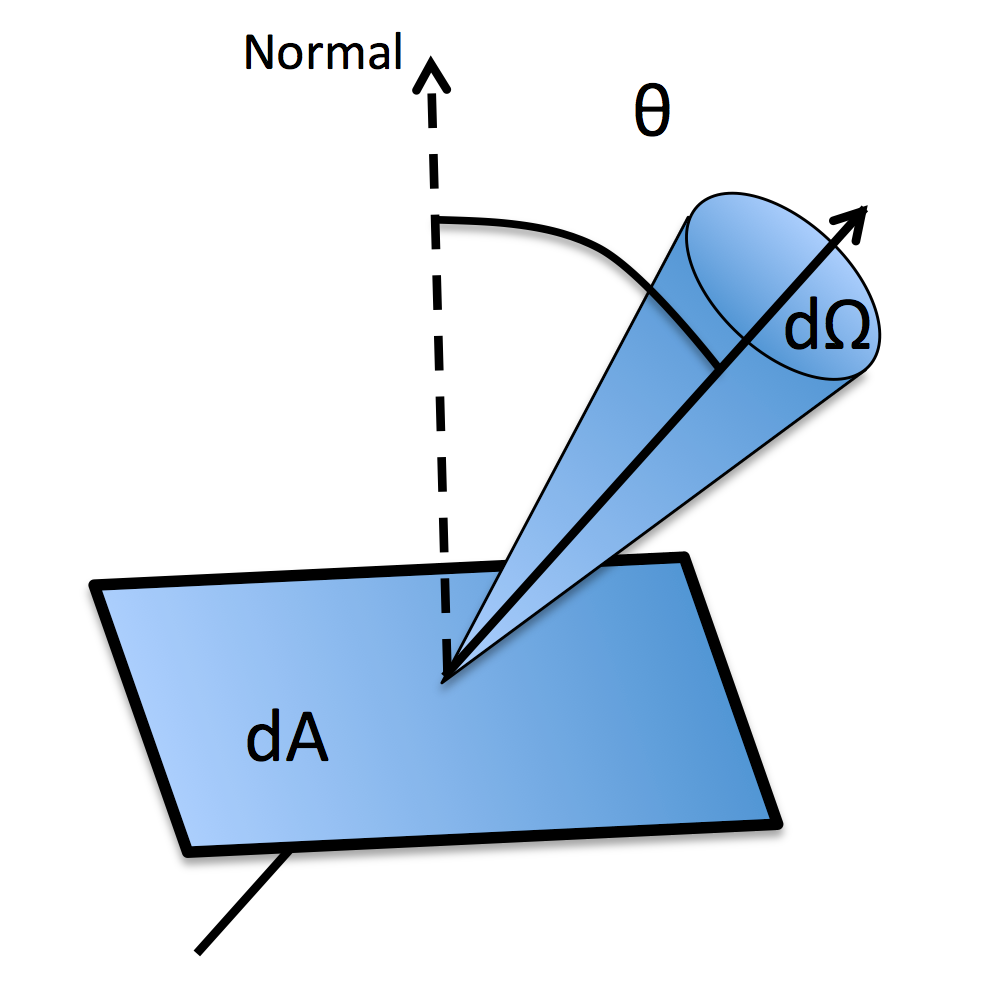
\includegraphics[width=0.5\textwidth]{figures/03-radtrans/rays_schematic.png}
\caption
{
A schematic showing a ray obliquely incident on a surface of area $dA$.
The labeled quantities are used in the definition of specific intensity.
} 
\label{fig:ray}
\end{figure}


The most fundamental quantity of radiative transfer is the 
{\em specific intensity}, $I_\nu$, defined as

\begin{equation}
I_\nu = \frac{dE}{d\Omega~dt~dA~d\nu},
\end{equation}

which has units of ${\rm erg~s^{-1}~Hz^{-1}~sr^{-1}~cm^{-2}}$.
By successively multiplying by $\cos \theta$ and integrating over solid angle we 
can obtain the first and second `moments' of the radiation field. These
are the flux, $F_\nu$ and momentum flux, $p_\nu$, respectively, given by

\begin{equation}
F_\nu = \int I_\nu \cos \theta~d \Omega,
\end{equation}

\begin{equation}
p_\nu = \frac{1}{c} \int I_\nu \cos^2 \theta~d \Omega
\end{equation}

We can also define the {\em mean intensity}, $J_\nu$, as

\begin{equation}
J_\nu = \frac{1}{4 \pi} \int I_\nu~d \Omega
\end{equation}

The mean intensity is particularly
useful when one wants to ignore the solid angle dependence of the radiation,
for example when considering the impact of an ionizing radiation field.

The equation describing the specific intensity change along a path element $ds$
is the radiative transfer equation, 

\begin{equation}
\frac{d I_\nu}{ds} = -\kappa_\nu I_\nu + j_\nu, 
\end{equation}

where $\kappa_\nu$ and $j_\nu$ are the absorption and emission coefficients respectively.
If we define the optical depth $d \tau_\nu = \kappa_\nu ds$ we can recast this as

\begin{equation}
\frac{d I_\nu}{d \tau_\nu} = -I_\nu + S_\nu
\label{eq:formal_rte}
\end{equation}

where $S_\nu=j_\nu/\kappa_\nu$ is the source function. This equation
is called the {\em formal radiative transfer equation}, and can be solved to give 

\begin{equation}
I_\nu = I_{\nu,0}~e^{-\tau_\nu} + \int^{\tau_\nu}_0 S_\nu (\tau^\prime_\nu)~e^{\tau^\prime_\nu-\tau_\nu} d \tau^\prime_\nu.
\label{eq:rte_solution}
\end{equation}

A useful limit is when the source function is constant in the absorbing medium, in which case
the integral can be easily evaluated to give

\begin{equation}
I_\nu = I_{\nu,0}~e^{-\tau_\nu} + S_\nu (1 - e^{-\tau_\nu}).
\label{eq:rte_solution}
\end{equation}

% The mean intensity, $J_\nu$ is a particularly useful quantity when calculation the ionization
% state 

\subsection{Spectral Line Formation}

From the above equations, it is trivial to show how emission and absorption lines form when
the source function is approximately constant.
Say we have a plasma illuminated by a blackbody of temperature $T_0$, such that
$I_{\nu,0} = B_\nu (T_0)$. The plasma layer then has a different temperature, $T$,
such that $S_\nu = B_\nu (T)$ in that medium. By inspecting equation~\ref{eq:rte_solution}
we can see that if we are optically thick within the line, but optically
thin in the continuum, then inside the line the source term is dominant and outside 
the line the first $I_{\nu,0}~e^{-\tau_\nu}$ term dominates. Therefore, if $T > T_0$ we will 
see an emission line, and if $T < T_0$ we will see an absorption line. 
This approach describes line emission in the blackbody limit; for more complicated SED shapes
it is necessary to construct simple model atoms.

\subsection{The Two Level Atom}

The two level atom formalism is well described by Mihalas (1978). 


\subsubsection{Einstein Coefficients}

Within the two level atom, the rate equation between the two levels in LTE can
can be written by invoking detailed balance, such that 
\begin{equation}
B_{lu} \bar{J}_{ul} n_l = B_{ul} \bar{J}_{ul} n_u + A_{ul} n_u,
\label{eq:rate_einstein}
\end{equation}
where $B_{ul}$, $B_{2ul}$ and $A_{ul}$ are the {\em Einstein coefficients}
for absorption, stimulated emission and spontaneous emission respectively.
The `mean intensity in the line', $\bar{J}_{ul}$, is given by
\begin{equation}
\bar{J}_{ul} = \int \phi(\nu) J_\nu d\nu.
\label{eq:jbar}
\end{equation}
In LTE, the level populations obey Boltzmann statistics, and thus we can also
write
\begin{equation}
\frac{n_l}{n_u} = \frac{g_l}{g_u} \exp (h \nu_{ul} / k_B T)
\end{equation}
We can then rearrange equation~\ref{eq:rate_einstein} in terms of the mean intensity,
and use the fact that, in LTE, $\bar{J}_{ul} = B_\nu (T)$ to write
\begin{equation}
\bar{J}_{ul} = (2 h \nu_{ul}^3) / c^2.
\end{equation}
Since this must be true at all values of $T$ we can also show that 
\begin{equation}
A_{ul} / B_{ul} = (2 h \nu_{ul}^3)~B_{lu} / B_{ul} = g_u / g_l
\end{equation}



\subsubsection{Collision Strengths}

As well as radiative excitation and de-excitation, bound electrons 
can also interact with the thermal pool of free electrons, meaning that
collisional rates also affect 




\subsection{The Sobolev Approximation}

The Sobolev approximation (SA) is a useful limit originally developed.
It is used to treat line transfer in fast-moving flows. Originally 
the theory was mostly applied to Stellar winds, although since then
a wide variety of astrophysical objects have been modelled using Sobolev treatments,
such as accreting systems (this work) and Supernovae.

The Sobolev limit is when the local bulk velocity gradients in a flow 
dominate other any thermal broadening. In the presence of these steep
velocity gradients, one can assume that the interaction of a ray with a bound-bound
transition takes place over a small resonant zone, known as a 
`Sobolev surface'. The length of this zone is defined by
\begin{equation}
l_s = \frac{v_{th}}{dv / ds}.
\end{equation}
It is important that the physical conditions of the c do not change on this scale.
If this is the case, then we can assume that all line interactions for a given 
frequency will occur at a single `resonant' point. The location at which
a given photon will interact with a line of frequency $\nu_{lu}$
is then given, in velocity space, by
\begin{equation}
v = c~\left(\frac{\nu}{\nu_{lu}} + 1\right).
\end{equation}
The Sobolev optical depth is then
\begin{equation}
d \tau = \frac{\pi e^2}{m c}  \left(n_l - n_u \frac{g_l}{g_u} \right) \frac{f_{lu} \lambda_{lu}}{c | dv / ds |}.
\end{equation}
We can see that the physical quantities determining line opacity are therefore 
the level populations in the plasma, the velocity gradient and the atomic physics
associated with the bound-bound transition.



\subsubsection{Escape Probabilities}





\subsection{Monte Carlo approaches}

Simple radiation transfer problems can be solved analytically,
but with more complicated geometries it is necessary to use Monte Carlo
techniques, which are easily solved with modern computing approaches and 
are intuitively parallelisable problems. I will describe one specific 
Monte Carlo radiative transfer (MCRT) code, which has been used
for the majority of the work in this thesis.

\section{{\sc python}: A Monte Carlo Ionization and Radiative Transfer Code}

\py\footnote{Named c. 1995, predating the inexorable rise of a certain widely used
programming language.} is a confusingly named 
Monte Carlo ionization and radiative transfer code. 
The general philosophy of the code is to be able to produce synthetic spectra
for astrophysical objects with outflows in 2.5D, using a self-consistent ionization 
treatment. The code is written in C, and has been in development since the mid-1990s.
Throughout this time it has been used with application to CVs \citep{LK02, M15},
YSOs \citep{simmacro2005}, Supernovae \citep{kerzendorfsim} and AGN/quasars 
\citep{higginbottom2013,H14,M16}. It is also capable of producing spectra 
for stellar winds and conducting simple photoionization balance calculations for
comparison with codes such as \textsc{cloudy}. Some more detail on code testing and 
development can be found in sections~\ref{sec:code_validation} and \ref{sec:code_maintenance}
respectively. Although the operation of \py\ is well-described by the above authors,
it is central to this Thesis and I will thus provide substantial detail on its operation. 

\subsection{Basics}

\begin{figure}
\centering
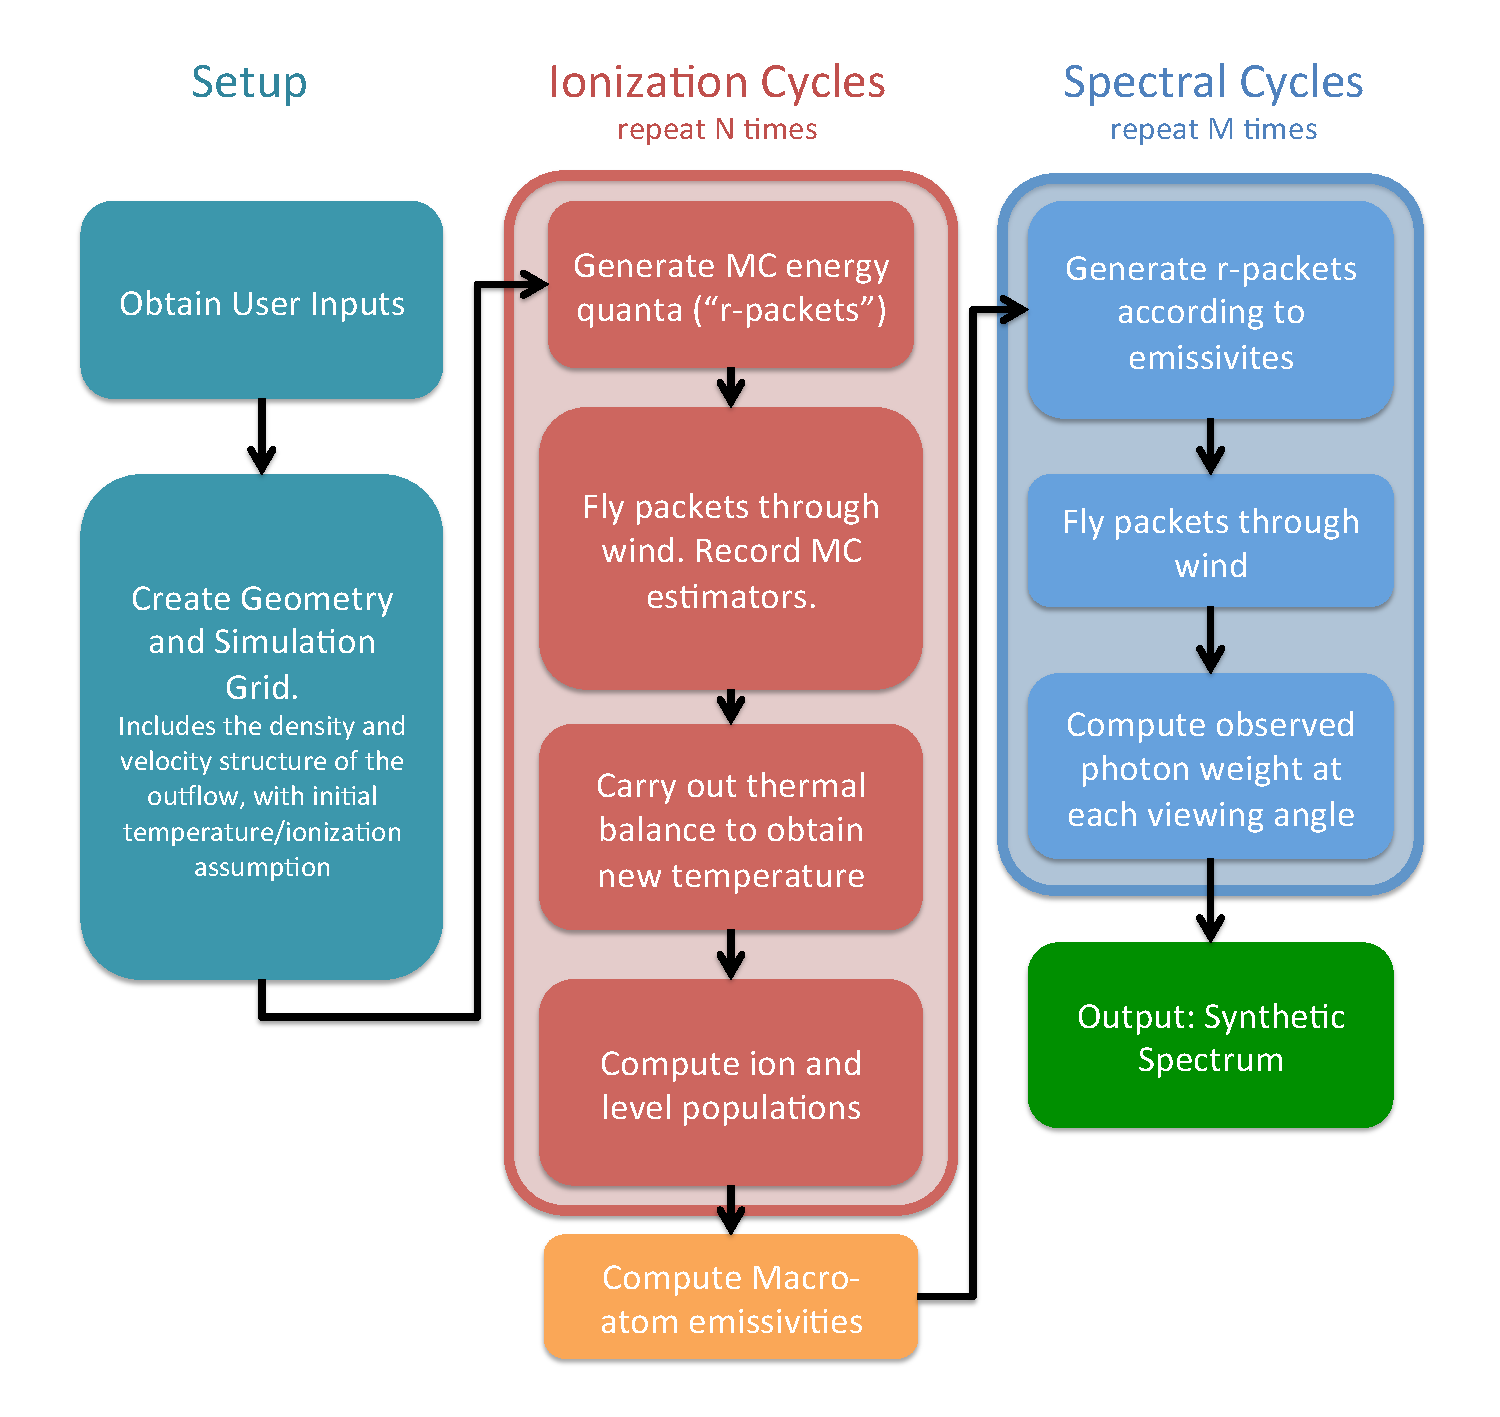
\includegraphics[width=1.0\textwidth]{figures/03-radtrans/flowchart.pdf}
\caption
{
A flowchart showing the basic operation of \py.
} 
\label{fig:flowchart}
\end{figure}

\py\ operates in three distinct stages, shown in figure~\ref{fig:flowchart}. 
First, the user specifies the photon sources,
geometry and kinematics of the system, normally with a similar parameterisation
to the SV93 model described in section~\ref{sec:sv93_model}. 
The code can operate with multiple coordinate systems 
(1D, spherical polar, cylindrical), but in this work I use cylindrical coordinates.
In this case, the outflow is discretised into a $n_x \times n_y$ logarithmic grid with 
user-specified dimensions. The co-ordinates, $(x_i, z_i$), 
of the corner of the $i$th cell are then given by
\begin{equation}
x_i = L_{x}~10^{(i-1)\frac{\log (R_{max} / L_{x})}{n_x}};~~
z_i = L_{z}~10^{(i-1)\frac{\log (R_{max} / L_{z})}{n_z}}, \\
\end{equation}
where $L_x$ and $L_z$ are appropriately chosen (but hardwired) scale lengths.
From these co-ordinates the poloidal distance can be calculated and
the velocity set according to equation~\ref{eq:v_law}. The density
is then calculated by imposing conservation of mass.

Once the basic setup process has been carried out, the ionization state,
level populations and temperature structure are calculated.
This is done via an iterative process, by transporting several populations of 
Monte Carlo energy quanta (`photons' or `$r$-packets) through the outflow.
This process is repeated until the code converges. 
In each of these iterations (`ionization cycles'), the code records estimators that 
characterize the radiation field in each grid cell. At the end 
of each ionization cycle, a new electron temperature is calculated
that more closely balances heating and cooling in the 
plasma. The radiative estimators and updated electron
temperature are then used to revise the ionization state of the wind,
and a new ionization cycle is started. The process is repeated until
heating and cooling are balanced throughout the wind. 

This converged model as the basis for the second set of
iterations (`spectral cycles'), in order to compute the synthetic spectrum based on the 
MC estimators record during the ionization cycles. 
The emergent spectrum over the desired spectral range is synthesized by 
tracking populations of energy packets through the wind and computing the emergent spectra at
a number of user-specified viewing angles.  

\py\ is designed to operate in a number of different
regimes, both in terms of the scale of the system and in terms of the
characteristics of the underlying radiation field.
It was originally developed by LK02 in order to model the UV spectra
of CVs with a simple biconical disc wind model. SDL05
\nocite{simmacro2005} used the code to model Brackett
and Pfund line profiles of H in young-stellar objects (YSOs). As part
of this effort, they implemented a `macro-atom' mode (see below) in
order to correctly treat H recombination lines with
\py. Finally, H13 used \py\ to model broad absorption line (BAL) QSOs. For
this application, an improved treatment of ionization was implemented,
so that the code is now capable of dealing with arbitrary
photo-ionizing SEDs, including non-thermal and multi-component ones. 


\section{Macro-atoms}

{\sl The macro-atom scheme was created by Leon Lucy and is outlined in 
his 2002/03 papers. It was implemented in \py\ by Stuart Sim, initially
for the study of recombination lines in YSO (Sim et al. 2005).}

Lucy (2002, 2003\nocite{lucy2002, lucy2003}; hereafter L02, L03) 
has shown that it is possible to calculate the emissivity of a gas in
statistical equilibrium without approximation for problems with large departures
from LTE.
% accurately by quantising matter into
% `macro-atoms', and radiant and kinetic energy into indivisible energy
% packets (r- and k- packets, respectively). 
His macro-atom scheme allows for all possible transition paths from a given level,
dispensing with the two-level approximation, and
provides a full non-local-thermodynamic-equilibrium (NLTE) solution
for the level populations based on Monte Carlo estimators. The macro-atom
technique has already been used to model Wolf-Rayet star
winds \citep{sim2004}, AGN disc winds \citep{simlong2008, tatum2012},
supernovae \citep{kromersim2009, kerzendorfsim} and YSOs (SDL05). A full 
description of the approach can be found in L02 and L03. 

The fundamental approach here requires somewhat of a philosophical shift.
Normally MCRT is described in the most intuitive way- that is, we imagine
real photons striking atoms and scattering, or photoionizing 
and depositing energy in a plasma. With Lucy's scheme we should instead 
reimagine the MC quanta as a packets of quantised energy flow, and the scheme as a 
{\em statistical} one. The amount of time a given energy quanta spends in a specific atomic
level or thermal pool is then somewhat analogous to the absolute energy 
contained therein.

Following L02, let us consider an atomic species interacting with a radiation field.
If the quantity $\epsilon_j$ represents the ionization plus excitation energy of 
a level i then the rates at which the level $j$ absorbs and emits radiant energy 
are given by

\begin{equation}
 \dot{A}_{j}^{R} = R_{\ell j} \epsilon_{j \ellp} \;\;\;\;\; and \;\;\;
\;\;  \dot{E}_{i}^{R} = R_{j \ellp} \epsilon_{j \ellp} \;\;\; ,
\end{equation}

Where I have adopted Lucy's convention in which the subscript 
$\ellp$ denotes a summation over all lower states.
Similarly, the rates corresponding to {\em kinetic} energy transport can then be written as

\begin{equation}
 \dot{A}_{j}^{C} = C_{\ellp j} \epsilon_{j \ellp} \;\;\;\;\; and
\;\;\;
\;\;  \dot{E}_{j}^{C} = C_{j \ellp} \epsilon_{j \ellp} \;\;\; ,
\end{equation}

If we now impose statistical equilibrium
%
\begin{equation}
 ({\cal R}_{\ellp j}-{\cal R}_{j \ell})+({\cal R}_{uj}-{\cal R}_{ju})=0 \;\;\;.
\end{equation}
 
we can then obtain 

\begin{eqnarray}
 \dot{E}_{j}^{R}+\dot{E}_{j}^{C}+{\cal R}_{ju}\epsilon_{i}+
 {\cal R}_{j \ell}\epsilon_{\ell}  \nonumber \\  
 = \dot{A}_{j}^{R}+\dot{A}_{j}^{C}+{\cal R}_{uj} \epsilon_{i}
 +{\cal R}_{\ell j} \epsilon_{\ell}           .  
 \label{eq:matom_SE}     
\end{eqnarray}

This equation is the starting point for the macro-atom scheme. It shows 
that, when assuming only radiative equilibrium, the energy flows through
a system depend only on the transition probabilities and atomic physics
associated with the levels the energy flow interacts with.
By quantising this energy flow into radiant (r-) and kinetic (k-) packets, 
we can simulate the energy transport through
a plasma discretised into volume elements (``macro-atoms''),
whose associated transition probabilities govern the interaction 
of radiant and kinetic energy with the ionization and excitation energy associated 
with the ions of the plasma.

Although equation~\ref{eq:matom_SE} assumes strict radiative equilbrium,
it is trivial to adjust it to include non-radiative source and sink terms. 
For example, in an expanding parcel of plasma, adiabatic cooling may be 
included with a simple modification to the RHS of equation~\ref{eq:matom_SE}.
%% XXX CHECK THIS.

% \subsection{Superlevels}
% One undesirable aspect of the macro-atom scheme is that the number of 
% jumps made inside a macro-atom can become large in certain limits.
% For example, when the plasma starts to approach LTE conditions
% the energy packets will spend a huge amount of time
% jumping between high up levels in a macro-atom. Fortunately, there
% are a number of fairly elegant solutions here. The first would be simply 
% to keep track of net rates-- if two large rates go in opposite directions
% but have a net difference, then all one needs to do is take account of that net
% difference and set the other rate to zero. This could be implemented in \py\, but
% is not currently. Instead, we adopt a method I shall refer to using the 
% term `superlevels'. 

% Once a cycle has been computed, it is possible to calculate departure coefficients, $D_j$
% for a level $j$, which are defined as

% \begin{equation}
% D_j = \frac{n_j}{n_j^{*,T_e}},
% \end{equation}

% which is simply the ratio of a level's population to it's LTE population at the electron temperature.
% If these coefficients approach unity at all levels above some threshold then these
% levels are said to be part of a superlevel. Any time we jump to a level $j$ inside a superlevel
% we instantly select a new level $k$ with a probability

% \begin{equation}
% P(j,k) = \frac{1}{N} \frac{n_j^{*,T_e}}{g_k} \sum_l P(k,l),
% \end{equation}
 
% where $1/N$ is just a normalisation over the sum of these quantities and $\sum_l P(k,l)$ represents 
% the sum of jumping probabilities to lower levels below the superlevel threshold.
% This formula produces the required jumping and deactivation distributions in the limit of LTE
% without having to actually go through the lengthy process of MC sampling the probability space.
% The speed-up can be huge in certain limits-- some models can undergo $\sim10^8$ jumps before deactivation,
% compared to an average of $\sim2$ in Lucy's original simulations.

\subsection{Macro-Atom Estimators}


\subsubsection{Radiation Field Estimators}

One of the most important estimators is the `mean intensity in the line', $\bar{J}_{lu}$,
which is defined by equation~\ref{eq:jbar}. 


\subsubsection{Heating And Cooling Estimators}

\subsection{Ionization Fractions and Level Populations}




\section{Simple-atoms}

% Prior to SDL05, the relative ionization fractions for all atomic
% species were estimated via the modified Saha equation (Mazzali \&
% Lucy 1993)  
% \begin{equation}
% \frac{n_{j+1} n_e}{n_j} = W [\xi + W(1-\xi)]
% \left(\frac{T_e}{T_R}\right)^{1/2}
% \left(\frac{n_{j+1}n_e}{n_j}\right)^*_{T_R}. \label{ionization}
% \end{equation}
% Here, the `starred' term on the right represents abundances computed with
% the Saha equation at temperature $T_R$, but using partition functions
% from the dilute blackbody approximation. 
% $W$ is an effective dilution factor, $\xi$ is the
% fraction of recombinations going directly to the ground state, and
% $T_R$ and $T_e$ are the radiation and electron temperatures,
% respectively. This simple ionization scheme produces reasonable
% results when the photoionizing SED can be approximated by a dilute
% blackbody. This is the case for high-state CVs. (As noted above, an
% improved, but more complex treatment of ionization that is appropriate
% for more complex SEDs is described in H13.) 

% Similarly, the relative excitation fractions within each ionization
% stage of a given species were estimated via a modified (dilute) Boltzmann
% equation,
% \begin{equation}
% \frac{n_{jk}}{n_j} = \frac{W g_k}{z_j(T_R)} \exp(-E_k/kT_R),
% \end{equation}
% where $n_{jk}$ is the population of level $k$ in ionic stage $j$,
% $E_k$ is the energy difference between level $k$ and the ground state,
% $g_k$ is the statistical weight of level $k$
% and $z_j(T_R)$ is the partition function of ionic stage $j$. 
% This equation is approximate, and in general this approximation 
% is not good. We therefore endeavour to treat any species in
% which the excitation state of the ions is thought to be important
% in determining either the ionizing radiation field, or emergent spectrum,
% as macro-atoms.

% Finally, \py\ originally modelled all bound-bound processes as transitions
% within a simple two-level atom \cite[e.g.][]{mihalas}. 
% This framework was used for the treatment of line transfer and also
% for the line heating and cooling calculations (see LK02). 
% The approximation works reasonably well for resonance  
% lines, such as \civfull, in which the lower level is the ground state.  
% However, it is a poor approximation for many other
% transitions, particularly those where the upper level
% is primarily populated from above. Thus an improved method for
% estimating excited level populations and simulating line transfer is
% needed in order to model recombination lines and continua.

\section{Heating And Cooling}

\subsection{Heating And Cooling Balance}

\subsection{Heating And Cooling Estimators}


Here I've tried to use Lucy's notation for macro-atom estimators. Take a three level system, in
which $l$ and $u$ represent lower and upper levels, 
and $\kappa$ represents the continuum level or upper ion.
q is the `absorption fraction' derived below, and $q_{ul}$ and $q_{lu}$ are the collisional
rate coefficients.

\subsubsection{Macro-atoms}

\noindent
In the macro-atom approach, we basically treat two communication pathways.
bound-free transitions represent a way
for radiant energy to communicate with the thermal pool
and bound-bound transitions represent a way
for excitation energy to communicate with the thermal pool.
\bigskip

\noindent
The heating and cooling rates for macro-atom bound-bound transitions are the rates of
collisional excitations and de-excitations
- i.e. the rate at which thermal energy is converted into
bound-bound excitation energy and vice versa.

\begin{equation}
C_{bb,matoms} = \sum_{lines} q_{lu} n_l n_e h \nu_{ul} V
\end{equation}

\begin{equation}
H_{bb,matoms} = \sum_{lines} q_{ul} n_u n_e h \nu_{ul} V
\end{equation}

\noindent
For bound-free transitions, we define the normal photoionization and recombination
rate coefficients $\gamma$ and $\alpha$, where $\alpha$ includes
stimulated recombination as we do in the code. Note
this differs to the approach in Lucy (2003), where it is instead included as a 
negative photoionization term, hence the notation $\widetilde{\gamma}$.
We also need to define two `modified rate coefficients' which 
are the rates at which b-f transitions add and remove energy to the radiation field.
These are denoted $\gamma^E$ and $\alpha^E$.

The rate at which recombinations convert
thermal {\em and} ionization energy into radiant energy is then
$\alpha^E h\nu_{\kappa l} n_\kappa n_e$, where $h \nu_{\kappa l}$ is the potential of the 
b-f transition, or the energy difference between continuum $\kappa$ and 
the level $l$ we are recombining too. 
The amount of this energy which is removed from the actual thermal pool
therefore needs a quantity $\alpha h\nu_{\kappa l} n_\kappa n_e$ subtracted from it,
giving
\begin{equation}
C_{bf,matoms} = \sum_{bf jumps} (\alpha^E - \alpha) n_e n_{\kappa}\nu_{\kappa l} V 
\end{equation}
where here I have also included stimulated recombination as we do in the code. Note
this differs to the approach in Lucy (2003), where it is instead included as a 
negative photoionization term, hence the notation $\widetilde{\gamma}$.
For photoionizations, we write a similar expression. The rate of at which
a level $l$ absorbs energy by b-f transitions is given by $\gamma^E h\nu_{\kappa l} n_\kappa n_e$,
but the amount $\gamma h \nu_{\kappa l} n_l$ goes into ionization energy, giving 
\begin{equation}
H_{bf,matoms} = \sum_{bf jumps} (\gamma^E - \gamma) n_l h \nu_{\kappa l} V
\end{equation}
as the rate at which radiant energy heats the plasma via b-f transitions.




\subsubsection{Simple-atoms}
\noindent
In simple-ions it is in some ways a little more complicated. 
First we define $q$ which will be different for each b-b transition, 
following Nick's thesis, which is given by 
(NB: I don't actually know how to derive this)
\begin{equation}
q = \frac{q_{ul} n_e (1 - e^{-h\nu/kT_e})}{\beta_{ul} A_{ul} + q_{ul} n_e (1 - e^{-h\nu/kT_e})}
\end{equation}
where $\beta_{ul}$ is the angle-averaged escape probability. 
$q$ represents {\em the probability that an excited bound electron
will collisionally de-excite}.
Our b-b heating rate is computed during the photon propagation and is a sum
over photons which come into resonance with each line, given by 
\begin{equation}
H_{bb,simple} = \sum_{photons} \sum_{lines} (1 - q) (1 - e^{-\tau_S}) w_{photon}
\end{equation}
And our bound bound cooling rate is given by 
\begin{equation}
C_{bb,simple} = \sum_{lines} q \left(n_l\frac{g_u}{g_l} - n_u\right) q_{ul} n_e 
\frac{(1 - e^{-h\nu/kT_e})}{(e^{h\nu/kT_e} - 1)}  h \nu_{ul}
\end{equation}
%%note the difference to the macro-atom approach- here this is already 
\noindent
The bound-free heating rate is given by
\begin{equation}
H_{bf,simple} = \sum_{photons} \sum_{bfjumps} w_{photon} e^{-\tau} \frac{\nu - \nu_{0}}{\nu}
\end{equation}
where $\nu$ here is the frequency of the photon in question, and $\nu_{0}$.
The bound-free cooling rate is then

\begin{equation}
C_{bf,simple} = ??
%%\sum_{bfjumps} \alpha_{sp} n_e n_{\kappa}
\end{equation}













\section{Spectral Synthesis}

The primary output from \py\ is a synthetic spectrum 
across a range of viewing angles. 
The code utilises a variance reduction technique in order to minimise the amount of 
time spent in the portion of the code. This technique is based 
on a similar method implemented by \citep{woods1991}.






A comparison between the two methods is shown in figure~\ref{fig:extract_demo}.

\begin{figure}
\centering
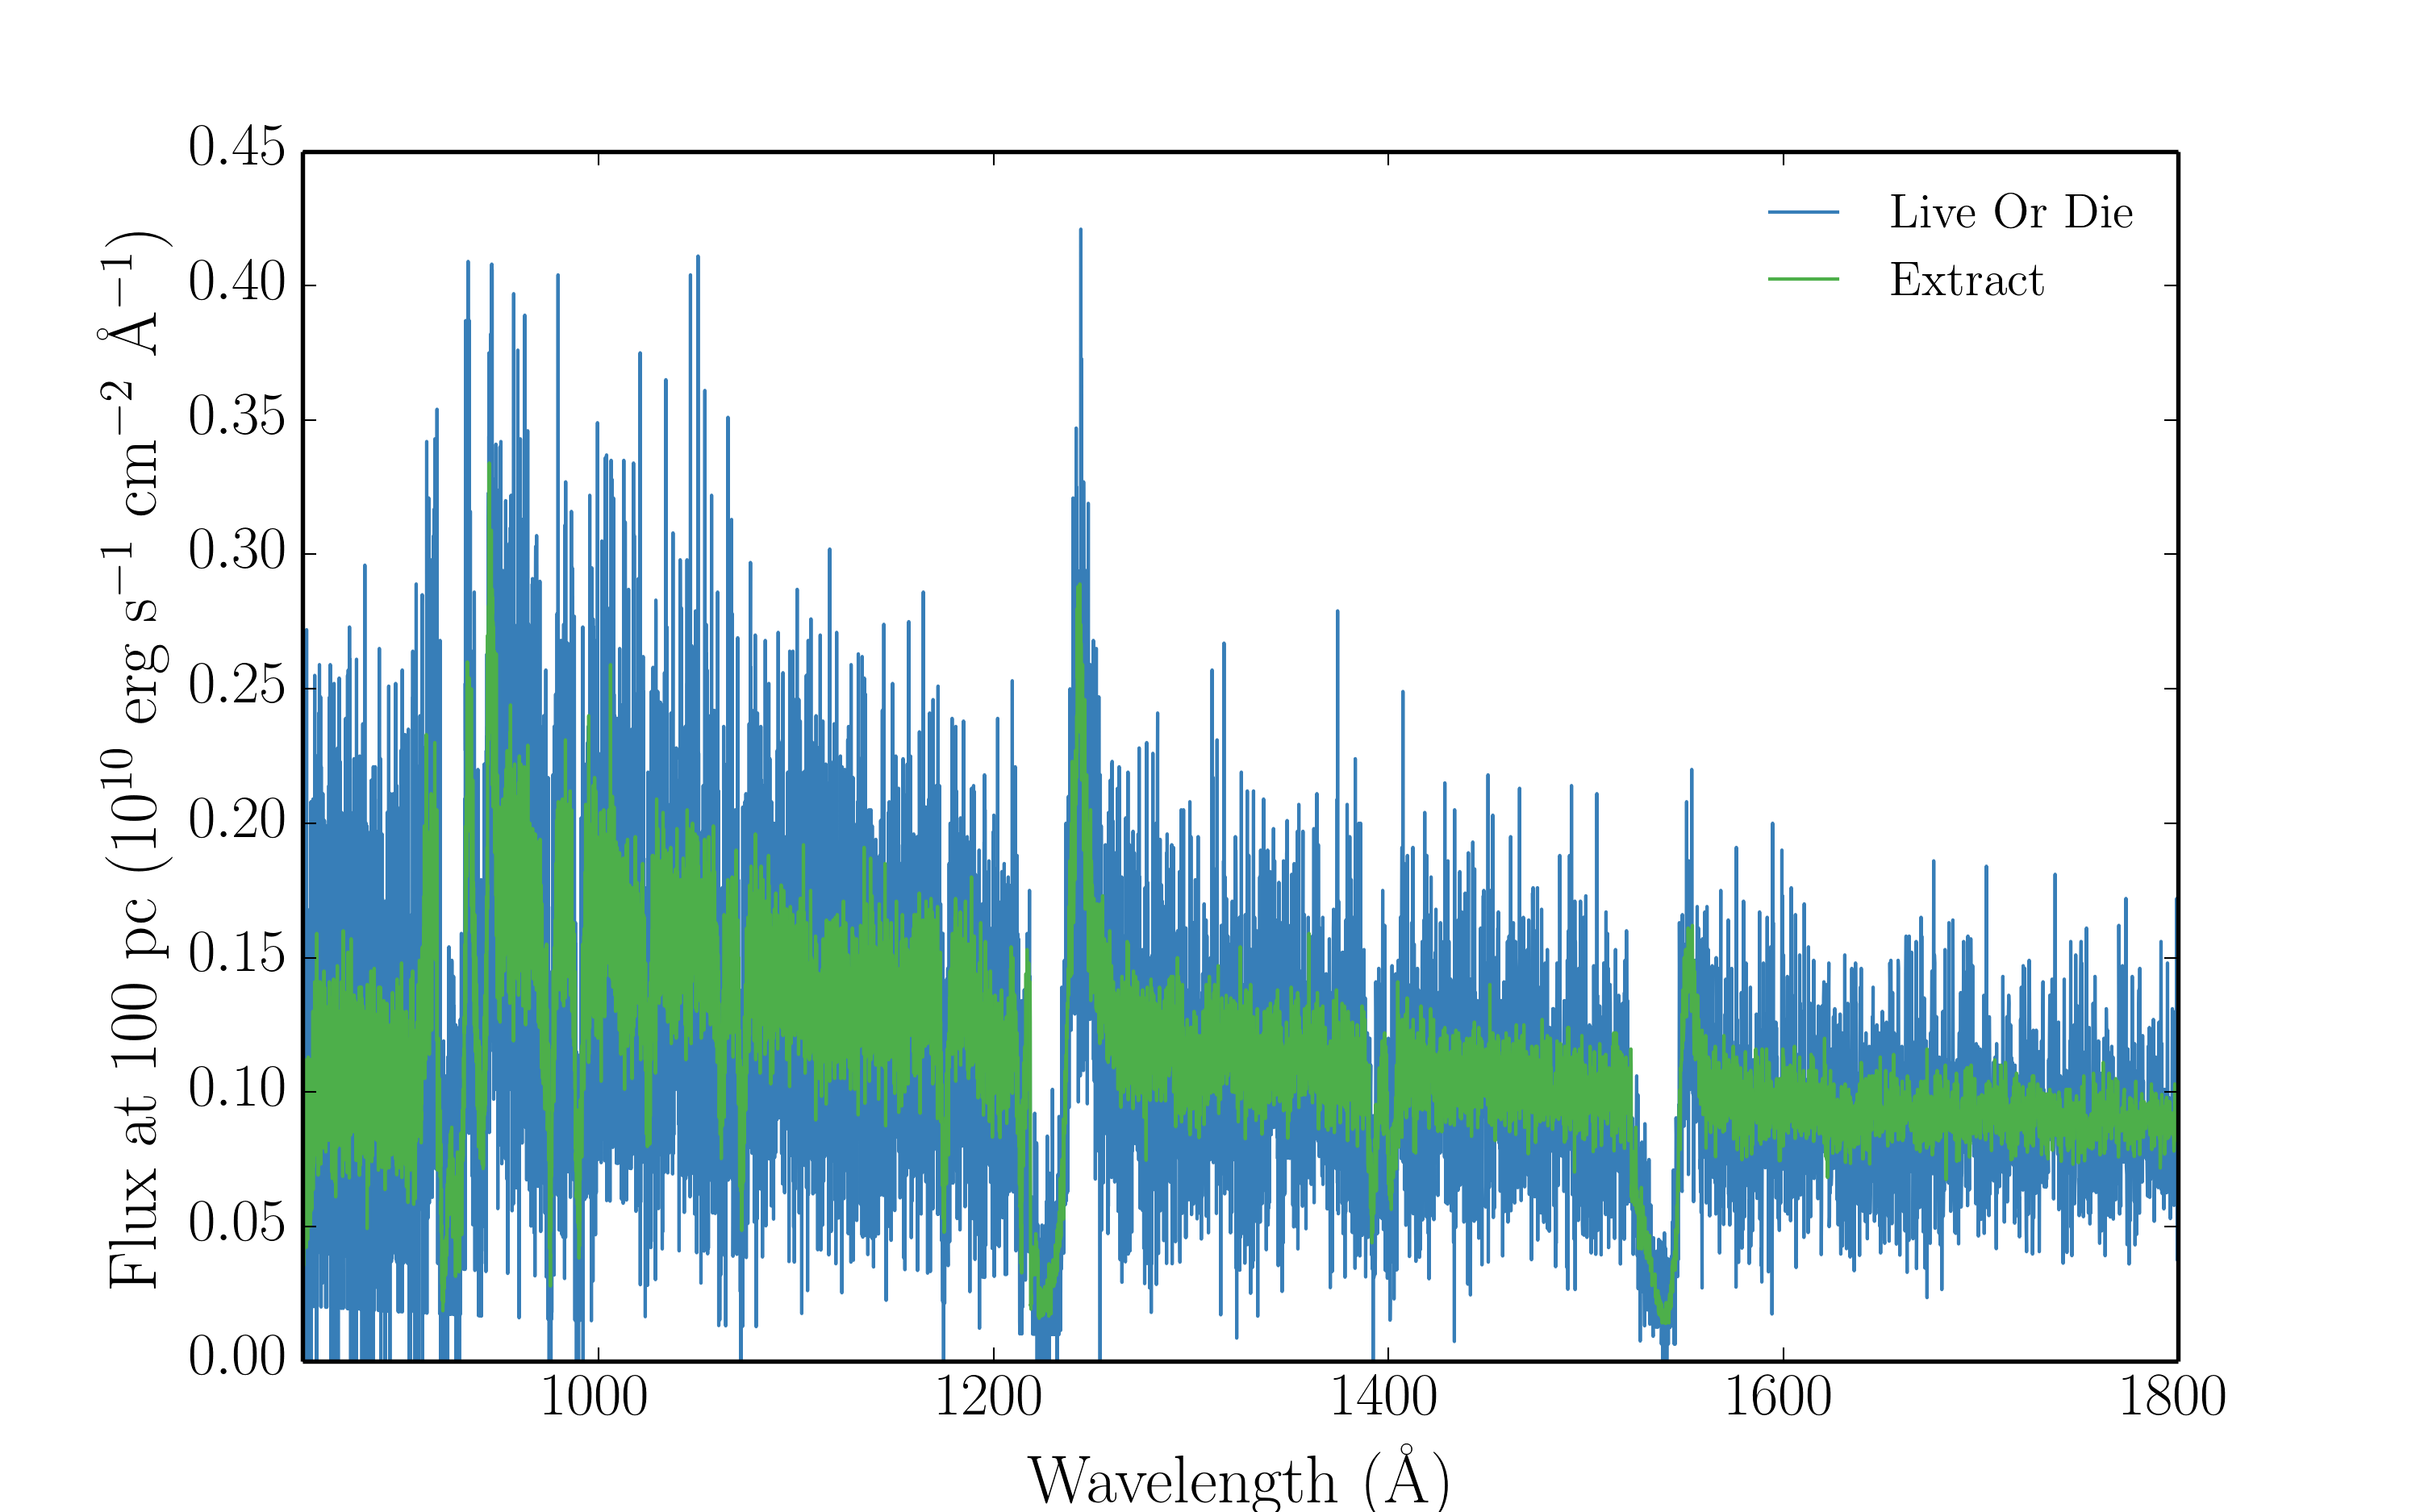
\includegraphics[width=1.0\textwidth]{figures/03-radtrans/extract_demo.png}
\caption
{
A Synthetic spectrum after $30$ spectral cycles with $100,000$ photons
from simple CV wind model at a $60^\circ$ viewing angle.
Spectra produced with both the extract and live or die modes
are shown. The effectiveness of the extract variance reduction technique can
be clearly seen, and we can see that the spectral shape is unaltered.
} 
\label{fig:extract_demo}
\end{figure}




\section{Atomic Data}

One of the big challenges in building reliable photoionization and radiative
transfer lies in the acquisition of accurate and complete atomic datasets.
All of the rates described so far contain a term, such as the oscillator strength 
or dimensionless collision strength, that is dependent purely on the atomic physics
associated with the transition. These quantities can be measured in laboratory experiments,
or predicted from atomic structure codes which derive the atomic physics from 
quantum theory.

Photoionization cross-sections are obtained from two sources. Where possible,
we use \top\ photoionization cross-sections. For macro-atoms,
these cross-sections are partial and represent the cross-section for a photoionization
from a given {\em level}. We neglect photoionizations to excited configurations
of the upper ion. For simple-atoms they are from the ground state.
The \top\ cross-sections have two major drawbacks in that 





\section{Clumping}

\label{sec:microclumping}

\subsection{Motivation}

As described in section~??, observational evidence for inhomogeneities in 
outflows is widespread. Clumping a plasma can have a significant effect on its
ionization, emission and absorption characteristics. Clearly, the interplay between
these effects will be somewhat complex 

A number of different implementations of clumping have been explored in previous studies,
mostly in the stellar winds community. Perhaps the simplest method is 
when one assumes that the individual clumps are both optically and geometrically thin;
this is known as {\em microclumping} \citep[e.g.][]{hamann1998,hilliermiller1999,hamann2008}. 
This technique has been particularly successful in reconciling discrepant mass-loss estimates.
It was found that one would obtain different mass-loss rates depending on whether
they were calculated from (i) UV resonance scattering of continuum photons 
(which scales linearly with density; a `$\rho$-diagnostic') or (ii) recombination 
and free-free emission process (which scale with the square of density; 
`$\rho^2$-diagnostics'). A clumped outflow would have enhanced densities in 
certain regions, and would thus mean that $\rho^2$-diagnostics tend to 
overestimate the total mass-loss rates. Microclumping has helped verify this
hypothesis with radiative transfer modelling (REFs). These clumpy models also
provide better fits to the electron scattering wings of emission lines in stellar
winds \citep{hillier1991}.

The second-generation of stellar wind codes went on step further by addressing the issue
of {\em porosity}; that clumps will have a finite size, and thus gaps between the clumps
may affect the emergent radiation field. This approach is known as {\em macroclumping}.
{\bf Describe macroclumping with references.}

Implementing a treatment of clumping in accretion disc wind models is challenging, for
two main reasons. First, the physical scale lengths and density contrasts 
in disc winds are not well-constrained from observations, especially in AGN.  
Second, there are significant computational difficulties associated with adequately
resolving and realistically modelling a series of small scale, high density
regions with a MCRT code. Given the lack of knowledge about the actual 
type of clumping, we encorporated the simpler microclumping approach into our code.
This is partly because our primary concern was the ionization and 
emission characteristics of the flow, and porosity was a secondary concern.


\subsection{Microclumping}

To take account of clumping in our outflow we adopt a simple parameterization
used in stellar wind modelling. The key assumption here is that typical clump sizes
are much smaller than the typical photon mean free path, and thus the clumps are 
both geometrically and optically thin. This approach is typically 
known as microclumping and allows one to introduce a `filling factor', $f$, which is the 
fraction of the volume of the plasma filled by clumps. We can then introduce the 
`density enhancement', $D$, which is simply 

\begin{equation}
D = \frac{1}{f}
\end{equation}

The densities in the model are then multiplied by this factor. This has the effect 
of enhancing `$\rho^2$' processes such as recombination or collisional excitation,
and 


\section{Code Validation}
\label{sec:code_validation}

The main challenge for high performance scientific computing can be 
elegantly summarised by Ferland's (2002) epitaph, {\sl `Reliability in the face 
of complexity'}. I have already delved into some of the complexity in this case,
so it is important to assess whether the code is also reliable before I present
results. 

\subsection{Testing against Cloudy}



\subsection{Testing against Tardis}


\section{Code Maintenance and Version Control}
\label{sec:code_maintenance}

As part of the expansion of the team working on \py\, I was responsible
for bringing the code under the auspices of a robust version control system.
Thanks to these efforts, the code is now hosted on GitHub at 
\url{https://github.com/agnwinds/python/}. Our team uses a Pull \& Fork model
for collaborative code development, in which major changes are made in a 
forked repository before the developer submits a `Pull request' to the main 
repository. To test the code, we use a combination of Travis CI build tests 
-- run per commit to the upstream repo -- and our own test suite which is 
run every night on a multi-core server. 

\begin{figure}
\centering
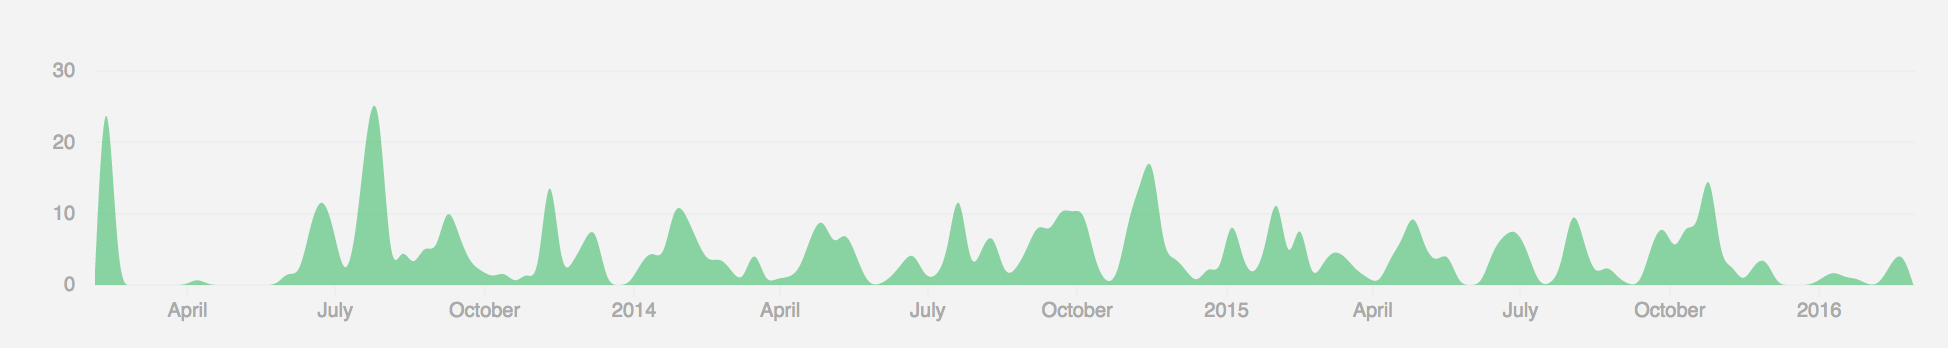
\includegraphics[width=1.0\textwidth]{figures/03-radtrans/github1.png}
\caption
{
Commit history from Feb 3, 2013 to Feb 29, 2016, showing the regular code development
that makes version control such a necessity to a collaborative code project. Produced
using the Github API and plotting capability.
} 
\label{fig:github}
\end{figure}

\subsection{Parallelisation} 










